\lab{Algorithms}{Value Function Iteration}{Value Function Iteration}

\objective{This section teaches the fundamentals of Dynamic Programming using value function iteration.}

Often it is of interest to optimize decision making in some sequential process.  For example, an oil company may need to decide how much oil to excavate and sell each month as prices change, a person entering retirement may need to decide how much of their savings to spend each year, or a model of economic growth may require a decision about how much to invest in capital versus how much to spend each year.  In this lab we will formulate a general dynamic optimization problem.  We will explore techniques for solving such a problem with both finite and infinite time horizons.

\section*{The Sequential Problem, Finite Horizon}\label{SecRecProbFinHor}
Suppose there are time periods $t=0,1,\ldots, T$ and at each time period we take an action $c_t$. Furthermore, at the beginning of each time period $t$ we are in some state $W_t$.  In many cases $W_t$ might represent an available resource, such as money.  At each time we receive some reward, $u(W_t,c_t)$, for taking action $c_t$ given state $W_t$.  We assume that rewards are worth more now than later. We let $\beta\in (0,1)$ represent what is called the discount factor and gives the ratio of preference for rewards today versus rewards tomorrow.  Lastly, over time our state variable $W_t$ changes according to some rule depending on the previous state and our actions,
\begin{equation}\label{motion}
W_{t+1} = g(W_t,c_t).
\end{equation}
Equation \eqref{motion} is sometimes referred to as the law of motion, as it describes how we move from state to state.
Mathematically such a problem can be represented as follows:
\begin{equation}\label{basic_prob}
\max \sum_{t=0}^T \beta^t u(W_t,c_t) \quad \text{s.t.} \quad W_{t+1} = g(W_t,c_t)
\end{equation}

where our initial state, $W_0$ is given.  There may also be restrictions on our choices $c_t$.  For example, in many applications the state $W_t$ represents the amount of some resource available, and $c_t$ represents the amount we use up in time period $t$.  In this case we would require $c_t \in [0,W_t]$.

For simplicity, lets assume that $u$ is a function of $c_t$ only (this is often, though not always, the case in practice).  First let's consider the case that $T=0$.  So we maximize
\begin{equation}\label{1perprob}
u(c_0)
\end{equation}
over $c_0 \in [0,W_0]$.  In most cases $u$ is increasing, which we will assume here.  In this case it will be optimal to choose the largest value of $c_0$ possible, that is, $c_0 = W_0$.  Thinking of $W_0$ as our available resources, this simply means, that if we don't have future periods to consider, we will use all of it.

In fact this is always true in the last period.  In the problem with $T$-periods we know that we will use all of our resources remaining in period $T$.  Consider the two period problem:
\begin{equation}\label{2perprob}
\max \, u(c_0) + \beta u(c_1)
\end{equation}
where $c_0 \in [0,W_0]$, $c_1 \in [0,W_1]$ and $W_1 = g(W_0,c_0)$.  We know that in the last period we will use all of our remaining resources so that $c_1 = W_1$.  Substituting gives
\begin{equation}
\max \, u(c_0) + \beta u(g(W_0,c_0)).
\end{equation}
Then we need only determine $c_0$.  Taking the derivative of \eqref{2perprob} with respect to $c_0$ and setting equal to zero gives the first order condition
\begin{equation}\label{FOC}
u'(c_0) = -\beta u'(g(W_0,c_0))g_c(W_0,c_0)
\end{equation}
where $g_c$ is the partial derivative of $g$ with respect to $c$.

Given a specific form for $u$ we could solve for $W_1$ and obtain the optimal solution.  In fact, we can solve a problem of any length $T$ in this manner by starting at the last time period and working backward.  We know that $W_{T+1} = 0$.  Working backward in time we obtain an equation at each time step $t<T$ by taking the derivative with respect to $c_t$ and setting equal to zero.  This process is called backward induction.  The equations at each time step, such as equation \eqref{FOC} are sometimes called the intertemporal Euler equations.  These equations, along with $c_T = W_T$ make $T+1$ equations to go with our $T+1$ unknowns $c_0,c_1,c_2,\ldots,c_T$ where we can use the law of motion to relate the $c_t$ and $W_t$.

\section*{The Recursive Problem, Finite Horizon}\label{SecRecProbFinHor}
Approaching the problem sequentially like this can be somewhat messy.  The dynamic programming approach we consider now is more easily adaptable to many situations.  The key to the dynamic programming approach is to define our optimization problem in terms of subproblems.  Notice that if we are in time period $t$, we face a problem of exactly the same form as the problem at time $0$.  We are in some state $W_t$, and want to maximize the sum from $t$ to $T$.  With this idea in mind, we define a function $V_t(W_t)$ called the value function.  The function $V_t$ gives the value of entering time $t$ in state $W_t$ and making optimal decisions moving forward.  So
\begin{equation}\label{value}
V_{t-1}(W_{t-1}) = \max u(c_{t-1}) + \beta V_t(g(W_{t-1},c_{t-1})).
\end{equation}
This is called the Bellman Equation.  The key to this formulation is that we decide what to do in period $t-1$ with the assumption that our actions in the remaining periods will be optimal.  This is called the principal of optimality.

Let us consider a specific example from economics called The Cake Eating Problem.  Suppose $W_t$ represents the size of a cake.  At each time period we can choose how much to consume.  What we eat,$c_t$, gives us rewards.  What we save,$W_t-c_t$, does not give rewards (until it is eaten in a later period).  The law of motion \eqref{motion} becomes
\begin{equation}\label{LOM_EX}
W_{t+1} = g(W_t,c_t) = W_t-c_t
\end{equation}
Now we have completely defined the problem.  The Bellman Equation is
\begin{equation}
V_{t-1}(W_{t-1}) = \max u(c_{t-1}) + \beta V_t(W_{t-1}-c_{t-1}).
\end{equation}
As before, we know that in the last time period, we should not save anything.  So $V_{T+1}(W_{T+1}) = 0$.  There is no value in leaving wealth for period $T+1$.  So $c_T = W_T$.  Then $V_T(W_T) = u(c_T)$.  Consider the value function equation for period $T-1$.
\begin{align}
V_{T-1}(W_{T-1}) &= \max u(c_{T-1}) + \beta V_T(W_{T-1}-c_{T-1}) \\
                 &= \max u(c_{T-1}) + \beta (W_{T-1}-c_{T-1}). \\
\end{align}

Thus given $W_{T-1}$, we can determine $V_{T-1}$ by maximizing over $c_{T-1}$.  Notice that by the law of motion, it is enough to determine the values of the $W_t$ since these determine the $c_t$.  In fact rearranging \eqref{LOM_EX} we have
\begin{equation}
c_t = W_t - W_{t+1}.
\end{equation}
Thus we can rewrite the value function as
\begin{equation}
V_{t-1}(W_{t-1}) = \max_{W_t} u(W_{t-1} - W_{t}) + \beta V_t(W_t).
\label{cake_valfn}
\end{equation}

The solution to this problem is often called a policy function.  A policy function determines an action based on the current state.  Denoting the policy function by $\psi$, this can be written
\begin{equation}
W_{t+1}=\psi_t \left(W_t\right)
\label{policy_fn}
\end{equation}
The policy function gives the optimal amount of cake to leave for next period (equivalent to the amount of consumption) given the amount of cake at the start of the period.  In other words, it determines the choice of $W_t$ that satisfies the $\max$ condition in equation \ref{cake_valfn}.

\begin{problem}  Follow the steps below to solve the problem described above.  Take $u(c_t) = \sqrt{c_t}$, $\beta = 0.9$, and $T=10$.
\begin{enumerate}
\item Let the maximum size of the cake be $W_{max} = 1$. Approximate the continuum of possible cake sizes by a column vector called $W$ that ranges from to 0 to 1.  Let the number of possible cake values be $N=100$.

   \item Note that in order to compute the value function we need $u(W_{t-1}-W_t)$.  Create an $N$ by $N$ matrix that contains all possible values of $W_{t-1} - W_t$ (where $W_{t-1}$ corresponds to rows and $W_{t}$ to columns).  Make sure that $c_t \geq 0$ is satisfied by replacing negative entries in the matrix with zero.  Then take the squareroot to get a matrix of $u(W_{t-1}-W_t)$.  To make sure we do not choose $W_{t-1} - W_t < 0$ when maximizing, replace the corresponding entries of the $u(W_{t-1}-W_t)$ matrix with a large negative number (e.g. $-10^{10}$).

   \item Next create an $N$ by $T+2$ (corresponding to $t=0,1,\ldots, T+1$) matrix representing the value function for a given time $t$ and state $W_t$.  We can initialize it to zeros and begin filling in the columns starting with the last (which we know is zeros).

   \item Now we are ready to iterate backward and find the value function for each time period.  To find $V_T$, we compute $u(W_T - W_{T+1}) + \beta V_{T+1}(W_{T+1})$ for all values of $W_{T-1}$ and $W_T$.  This will result in an $N$ by $N$ matrix where the rows correspond to values of $W_{T}$ and the columns correspond to values of $W_{T+1}$.  Note that to compute this we need a matrix representing $\beta V_{T+1}(W_{T+1})$.  Because this quantity does not depend on $W_T$, its rows should be equal.  To do this, we want to take $\beta V_{T+1}(W_{T+1})$ as a row vector and stack this vector to create a matrix with equal rows.  There are multiple python functions that can be used to achieve this.  One is the repeat function.  For example, if b is a row vector it could be used like the following.

       \begin{lstlisting}
       In [644]: b = sp.array([[1,2,3]])

       In [645]: b
       Out[645]: array([[1, 2, 3]])

       In [647]: sp.repeat(b,3,axis = 0)
       Out[647]:
                array([[1, 2, 3],
                [1, 2, 3],
                [1, 2, 3]])
       \end{lstlisting}

       In general, be careful about having the correct rows,columns, transposes, etc throughout your code.

       Now we maximize over choices of $W_T$ (choosing how much to save for next period).  Then we will have a row vector representing the value function for period $T$ across all possible $W_T$.  Iterate this procedure to fill in the value function for all $t=0,1,\ldots, T+1$.

   \item In each iteration you maximize to find the value function at time $t$.  Save the values of $W_{t+1}$ that achieve the maximum.  The result is an $N$ by $T+1$ matrix whose $n,t$ entry gives the optimal amount of cake to leave for for period $t+1$ given that we start period $t$ with the the $n$th value of our $W$ vector of cake.  This is the policy function.

   \item Plot the surface of the Value and Policy functions.  This can be done by including the following import lines

        \begin{lstlisting}
        from matplotlib import pyplot as plt
        from matplotlib import cm
        from mpl_toolkits . mplot3d import Axes3D
        \end{lstlisting}

        and using the following code

        \begin{lstlisting}
        x=sp.arange(0,N)
        y=sp.arange(0,T+2)
        X,Y=sp.meshgrid(x,y)
        fig1 = plt.figure()
        ax1= Axes3D(fig1)
        ax1.plot_surface(W[X],Y,sp.transpose(V), cmap=cm.coolwarm)
        plt.show ()

        fig2 = plt.figure()
        ax2 = Axes3D(fig2)
        y = sp.arange(0,T+1)
        X,Y=sp.meshgrid(x,y)
        ax2.plot_surface(W[X],Y,sp.transpose(psi), cmap = cm.coolwarm)
        plt.show()
        \end{lstlisting}

        where W is the vector of wealth levels, V is the value function, and psi is the policy function.

        You should also try plotting the value and policy functions for fixed time periods across $W_t$, or for fixed $W_t$ across time and make sure that these plots fit your intuition.

\end{enumerate}
\end{problem}

\begin{figure}
\centering
\begin{subfigure}{.5\textwidth}
    \centering
    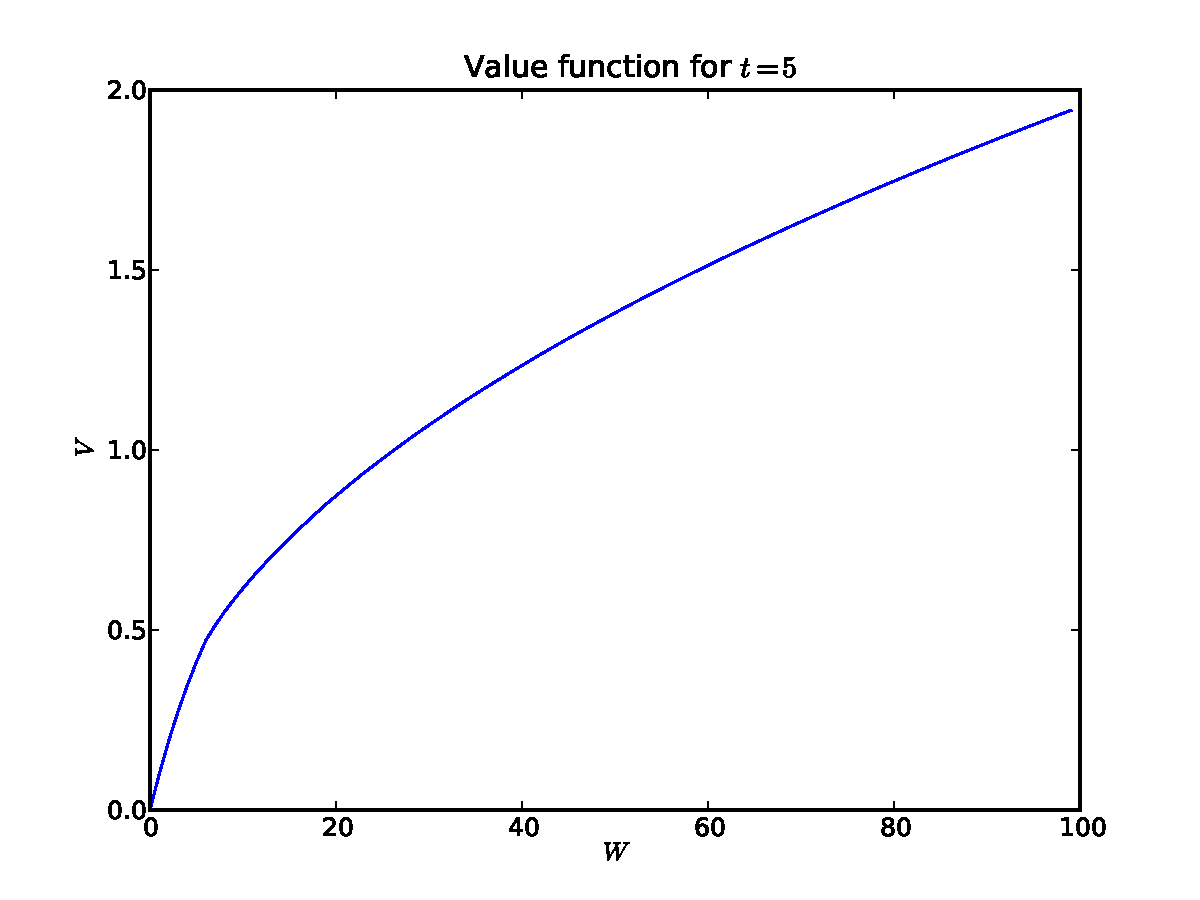
\includegraphics[width=\textwidth]{fixed_time.pdf}
\end{subfigure}%
\begin{subfigure}{.5\textwidth}
    \centering
    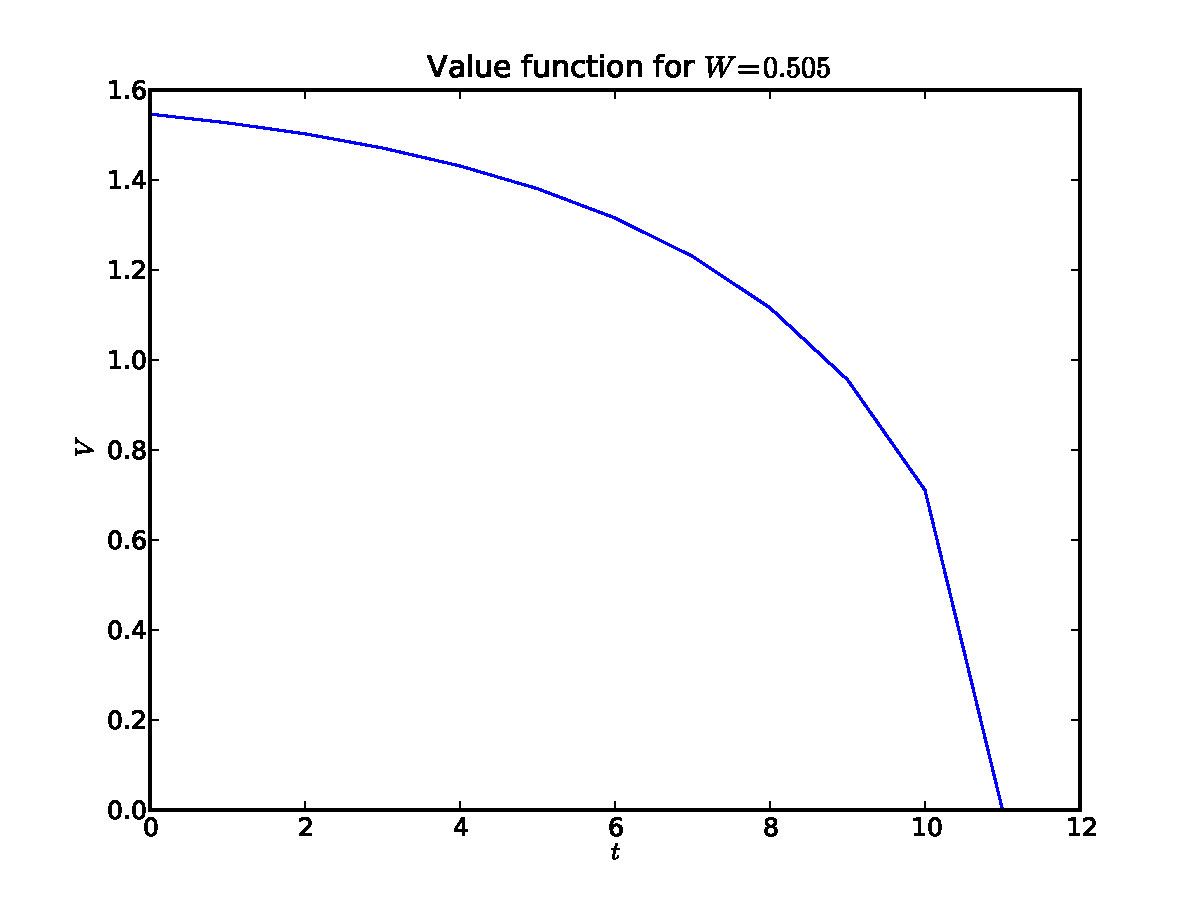
\includegraphics[width=\textwidth]{fixed_w.pdf}
\end{subfigure}
\caption{Slices of the finite horizon value function for fixed values of $t$ and $W$.}
\end{figure}

\section*{The Recursive Problem, Infinite Horizon}\label{SecRecProbInFHor}
Next we consider an infinite horizon problem.  For simplicity, we continue with the example from the previous section.  Suppose that rather than optimizing over $t = 0,1,\ldots,T$, we wish to optimize over an infinite time horizon:
\begin{equation}\label{inf_prob}
\max \sum_{t=0}^\infty \beta^t u(W_t,c_t) \quad \text{s.t.} \quad W_{t+1} = g(W_t,c_t).
\end{equation}
Since at any time $t$, there are an infinite number of periods remaining, one might suspect that the optimal policy will not depend on the current time $t$.

\begin{problem}
Compute the solution to Problem 1 with $T = 1000$.  Plot the policy function across time for fixed $W_t = 1$.  Notice that it is the same for all time periods, except those near the end time $T$.
\end{problem}

As suggested by the results of Problem 2,  the policy function for the infinite horizon problem does not depend on the time $t$ (this can be proved).  That is, at any time $t$, the optimal decision depends only on the amount of cake at the beginning of the period, not the value of $t$.  So everything can now be written in terms of variables today and variables tomorrow. We will denote variables tomorrow with a ``$\:'\:$".
\begin{equation}\label{EqBellman}
   V\left(W\right) = \max_{W'\in[0,W]}\:\: u\left(W - W'\right) + \beta V\left(W'\right)
\end{equation}
Note that the value function $V$ on the left-hand-side of \eqref{EqBellman} and on the right-hand-side are the same function.

Because the problem now has an infinite horizon, the nature of the solution is a little different. The solution to \eqref{EqBellman} is a policy function $W'=\psi(W)$ that creates a fixed point in $V$. In other words, the solution is a policy function $\psi(W)$ that makes the function $V$ on the left-hand-side of \eqref{EqBellman} equal the function $V$ on the right-hand-side.

Define $C$ as an operator on any value function $V_k\left(W\right)$. Let $C$ perform the following operation.
\begin{equation}\label{EqContraction}
   C\Bigl(V_k\left(W\right)\Bigr) \equiv \max_{W'\in[0,W]}\: u\left(W-W'\right) + \beta V_k\left(W'\right)
\end{equation}
Note that the value function on the right-hand-side of \eqref{EqContraction} and on the left-hand-side are the same function $V_k$, but have a different value of the size of the cake---$W$ versus $W'$. The operator $C$ takes in a function $V_k$, and gives a new function which we will call $V_{k+1}$:
\begin{equation}\label{EqContractionV}
   V_{k+1}\left(W\right) \equiv C\Bigl(V_k\left(W\right)\Bigr).
\end{equation}
The value function $V_{k+1}$ that results from the operation $C$ is not necessarily the same as the value function that the system began with $V_k$. However, according to equation \eqref{EqBellman} we seek a $V$ such that $C(V) = V$.  The solution, then, is the fixed point in $V$.
\begin{equation}
   C\Bigl(V_k\left(W\right)\Bigr) = V_{k+1}\left(W\right) = V_k\left(W\right) = V\left(W\right)
\end{equation}

The operator $C(\cdot)$ is called a contraction mapping if applying it over and over again to an arbitrary value function $V_k$ converges to a fixed point. One way to characterize a contraction mapping is:
\begin{equation}
   \lim_{k\rightarrow\infty}\: C^k\Bigl(V_0\left(W\right)\Bigr) = V_k(W) =  V\left(W\right)
\end{equation}
for any $V_0$.  It can be shown that if $u(\cdot)$ is real-valued, continuous, and bounded, $\beta\in(0,1)$, and that the constraint set $W'\in[0,W]$ is nonempty, compact-valued, and continuous, then the operator $C$ is a contraction and thus we can obtain a solution by iteration.

Remember, in the infinite horizon problem both the value and policy functions do not depend on time.  Computationally, this means that the value and policy functions in the infinite horizon problem are one dimensional.

\begin{problem}
Solve The Cake Eating Problem with an infinite time horizon by following the steps below.  As in Problem 1, take $u(c_t) = \sqrt{c_t}$, $\beta = 0.9$.
\begin{enumerate}
   \item As in Problem 1, let the maximum size of the cake be $W_{max} = 1$. Approximate the continuum of possible cake sizes by a column vector called $W$ that ranges 0 to 1.  Let the number of possible cake values be $N=100$.

   \item  Initialize the value function, V to a vector of zeros of length $N$.  This is $V_0$  Perform one iteration of the contraction operation given in equation \eqref{EqContraction} to get a new value function $V_1$ (this should be very similar to Problem 1).  Determine the resulting policy function $W' = \psi_1\left(W\right)$.  [HINT: The policy function should be a vector of length $N$ of optimal future values of the cake $W'$ given the current value of the cake $W$, and $V_T$ should be an $N$-length vector representing the value of entering a period with cake size $W$.]

   \item Generate a norm $\delta_0 = \norm{V_0\left(W\right) - V_1\left(W'\right)}$ that measures the distance between the two value functions. Define the distance metric as the sum of the squared differences,
   \begin{equation}\label{EqDist}
      \delta_1\equiv \norm{V_1\left(W\right) - V_0\left(W'\right)} = \left(V_1 - V_0\right)'*\left(V_1 - V_0\right)
   \end{equation}
   where $\left(V_1-V_0\right)'$ is the transpose of the difference of the two vectors. Defined in this way, $\delta_1\in [0,\infty)$.

   \item Take the resulting $V_1$ from (b), and perform the same contraction on it to generate $V_2$ and $\psi_2$. That is, generate,
   \begin{equation*}
      V_2\left(W\right) = C\Bigl(V_1\left(W\right)\Bigr) = \max_{W'\in[0,W]}\: u\left(W - W'\right) + \beta V_1\left(W'\right)
   \end{equation*}
   and the accompanying policy function $W'=\psi_2\left(W\right)$. Calculate the accompanying distance measure for $\delta_2$ using the formula from \eqref{EqDist} with the updated period subscripts. Compare $\delta_2$ with $\delta_1$ from (c).

   \item Repeat (d) and generate $V_3$ and $\psi_2$ by performing the contraction on $V_2$. Compare $\delta_3$ to $\delta_2$ and $\delta_1$.

   \item Write a loop that performs the contraction operation from (b), (d), and (e) iteratively until the distance measure is very small $\delta_k < 10^{-9}$.  The distance measure $\delta_k$ being arbitrarily close to zero means you have converged to the fixed point $V_k = V_{k+1} = V$. (For fun, you can show that the policy function converges to the same function regardless of what you put in for your initial policy function value.)

   \item Plot the policy function for the converged problem $W' = \psi\left(W\right)$ which gives the value of the cake tomorrow ($y$-axis) as a function of the cake today ($x$-axis).

\end{enumerate}
\end{problem}

\begin{figure}
    \centering
    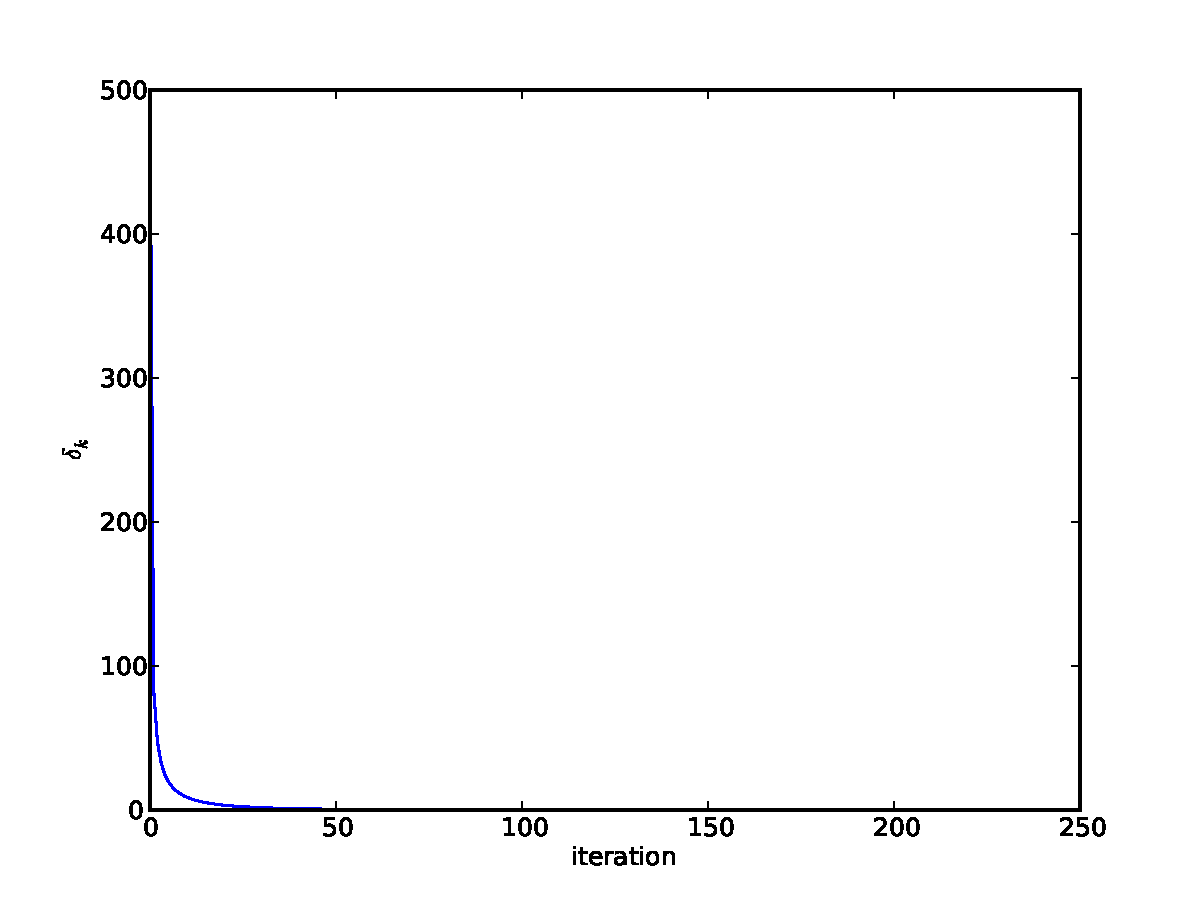
\includegraphics[width=\textwidth]{convergence.pdf}
    \caption{Due to the contraction mapping principle, $\delta_k$ decreases as we perform iterations until it is small enough to meet our convergence tolerance.}
\end{figure}
